In \autoref{fig:simpleThreeLatticeIsing} two examples of lattice-shapes were already introduced.
In the research leading to this thesis, a selection of lattices were chosen.
The implementation supports a 1D lattice (the default \textbf{linear} lattice/chain  (\autoref{fig:appendix-linear-lattices})) and five different 2D lattices 
(\textbf{cubic} (\autoref{fig:appendix-cubic-lattices}), \textbf{hexagonal} (\autoref{fig:appendix-hexagonal-lattices}), \textbf{trigonal\_square} (\autoref{fig:appendix-trigonal_square-lattices}), \textbf{trigonal\_hexagonal} (\autoref{fig:appendix-trigonal_hexagonal-lattices}) and \textbf{trigonal\_diamond} (\autoref{fig:appendix-trigonal_diamond-lattices})).

The lattice structure can be interactively visualized with the use of \cite{selfPhysics} \filepath{/structures/visualize.py}.
The same code was used to generate the referenced visualization printed in the \nameref{sec:appendix}.

The numbers, that can be seen in the visualization denote the location-index of the memory, that is responsible for carrying the spin state at that lattice site in the later representation. As will become obvious in \fullref{sec:theory-graphs}, the structure of a lattice cannot always be represented directly analogous in memory. Therefore an alternative way of addressing lattice sites and theirs surroundings needs to be employed.
In this case, the framework generates the set of \emph{nearest neighbor} (marked green in the visualization) and \emph{next-nearest neighbor} (marked yellow in the visualization) indices for a given lattice site (marked red in the visualization). These are used as structural inputs for later discussed \emph{graph} architectures.

A quite important feature for the physical aspect of the calculation is the \emph{periodicity} of a lattice. 
As real world crystals have many magnitudes more lattice sites than can be simulated currently, \emph{boundary effects} play a significant role in simulated latices.
This often times is an unwanted manner, if the goal is to calculate the behavior of the system far away from the edges. 
Lattices should there have the property of \emph{translational symmetry}. 
To aid with this, a \emph{periodic} repetition of the lattice can be toggled. 
It is responsible for defining neighbors for lattice sites close to the edges of the lattice.
The \nameref{appendix:lattice-visualisation} in the appendix shows this, by providing the information whether the pictured lattice is periodic or not.

The way in that the lattices are tiled is should become clear from the visualization.
It is noteworthy, that the \textbf{cubic}, \textbf{trigonal\_square} and \textbf{trigonal\_diamond} lattices have repetition along two axes, while the \textbf{hexagonal} and \textbf{trigonal\_hexagonal} have three. 
The hope is that the \textbf{trigonal\_hexagonal} and \textbf{trigonal\_square}/\textbf{trigonal\_diamond} lattices show the same behavior in non-periodic mode (as they all three represent a trigonal lattice), while differences manifest in periodic inspection.

Last, there is a setting to \emph{randomly swap} lattice positions. 
The effect of this can be seen in \autoref{fig:direct-comparison-lattice-site-swaps}.

\begin{figure}[htbp]
    \centering
    \makebox[\textwidth][c]{
        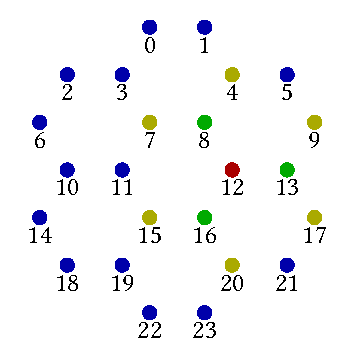
\includegraphics[width=0.3\textwidth]{./theory/physics/explored-lattice-patterns/hexagonal,size=2,np.pdf}
        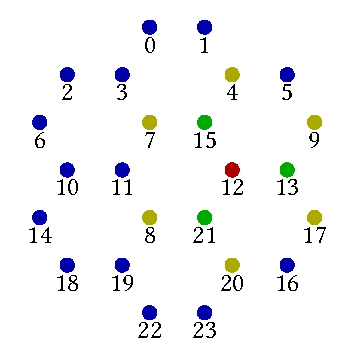
\includegraphics[width=0.3\textwidth]{./theory/physics/explored-lattice-patterns/hexagonal,size=2,np,rs=2.pdf}
    }
    \makebox[\textwidth][c]{
        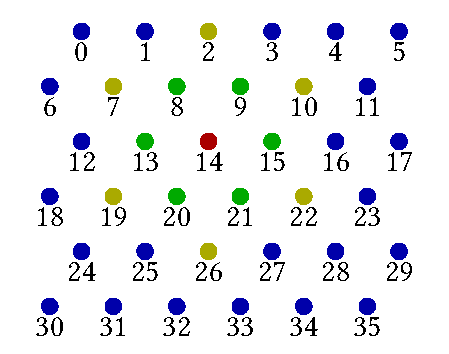
\includegraphics[width=0.3\textwidth]{./theory/physics/explored-lattice-patterns/trigonal_square,size=3,np.pdf}
        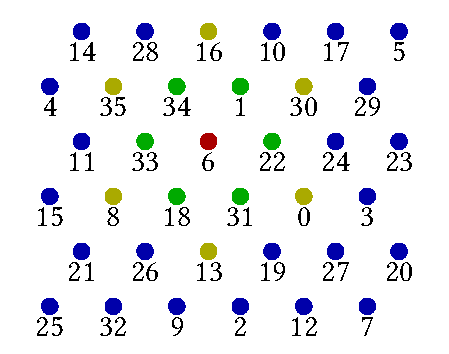
\includegraphics[width=0.3\textwidth]{./theory/physics/explored-lattice-patterns/trigonal_square,size=3,np,rs=-1.pdf}
    }

    \vspace{0.2cm}
    \caption{Visualization of the property \emph{random swaps} of the lattice structure helper. In the first set of figures, two swaps were performed on a hexagonal lattice of size 2 (8 with 15 and 16 with 21). The neighbor-index calculation takes this into effect, therefore the highlighted lattice sites do not change. The second set of figures shows the setting -1 for a trigonal\_square lattice of size 3. This basically makes the generator perform such a high number of pair swaps, so that the index-position correlation can be taken as randomly. 
    }
    \label{fig:direct-comparison-lattice-site-swaps}
\end{figure}

The goal of this setting is to decouple the in-memory representation and the structure of the simulated lattice. 
Effects of this will be explored in \fullref{sec:experiments-resiliencylatticeencoding}.

General data about the lattices is provided in \autoref{table:lattice-information}.

\begin{table}[htbp]
    \centering
    \begin{tabular}{l|cc|ccccccc} 
        \toprule
        Lattice name & \#nn & \#nnn &$L$(1)&$L$(2)&$L$(3)&$L$(4)&$L$(5)&$L$(6)&$L$(7)\\  
        \midrule 
        linear & 2 & 2 & 1 & 2 & 3 & 4 & 5 & 6 & 7\\
        cubic & 4 & 4 & 4 & 9 & 16 & 25 & 36 & 49 & 64\\
        trigonal\_square & 6 & 6 & 4 & 16 & 36 & 64 & 100 & 144 & 196\\
        trigonal\_diamond & 6 & 6 & 4 & 9 & 16 & 25 & 36 & 49 & 64\\
        trigonal\_hexagonal & 6 & 6 & 7 & 19 & 37 & 61 & 91 & 127 & 169\\
        hexagonal & 3 & 6 & 6 & 24 & 54 & 96 & 150 & 216 & 294\\
        \bottomrule
    \end{tabular}
    \vspace{0.5cm}
    \caption{General information about the explored lattices. \textbf{\#nn} describes the number of nearest neighbors, \textbf{\#nnn} the number of next nearest neighbors. The numbers describe the maximum possible neighbor count. If a lattice is non-periodic, some sites can have less neighbors. $L(i)$ describes the number of lattice sites for a lattice of \textbf{size=$i$}}
    \label{table:lattice-information}
\end{table}

% TODO SOURCE: \cite{hexagonalGrids}




